\documentclass[10pt, fleqn, dvipdfmx]{article}

\usepackage{amsmath}
\usepackage[top=3cm, bottom=3cm, left=1cm, right=1cm]{geometry}
\usepackage{listings}
\usepackage{xcolor}
\usepackage{graphicx}

\lstset{
	basicstyle=\ttfamily\small,
	frame=single,
	breaklines=true,
	postbreak=\mbox{\textcolor{red}{$\hookrightarrow$}\space},
	columns=fullflexible,
	numbers=left,
	xleftmargin=2.5em,
	framexleftmargin=2em
}
\renewcommand{\figurename}{図}

\DeclareRobustCommand{\rchi}{{\mathpalette\irchi\relax}}
\newcommand{\irchi}[2]{\raisebox{\depth}{$#1\chi$}}

\parindent = 0pt

\begin{document}

\begin{center}
	{\Huge システム数理特別講義Ⅱ}
\end{center}

\begin{flushright}
	{\Large \today ~~~~ 29C23002 ~~~ 石川健太郎}
\end{flushright}

\section*{(1)}

\begin{align}
	\left\{
	\begin{aligned}
		 & \dot{x}(t) = A x(t) + B u(t), \\
		 & x(0) = x_0,                   \\
		 & y(t) = C x(t).
	\end{aligned}
	\right.
	\label{fom1-1}
\end{align}

式 \eqref{fom1-1} から, 基準の時間を $t_0$ として次が得られる.

\begin{equation}
	x(t) = e^{A (t - t_0)} x(t_0) + \int_{t_0}^t e^{A (t - \tau)} B u (\tau) d\tau
\end{equation}

$T$ をサンプル時間, $k$ を非負の整数とする.

$kT \leq t \leq (k+1)T$ で $u(t) = u_k$ という定数の入力 (0 次ホールド) が加えられる.

$t_0 = kT, ~~ t = (k+1)T$ として, $x((k+1)T)$ を考える.

\begin{align}
	x((k+1)T)
	 & = \exp \left( A ((k+1)T - kT) \right) x(kT)
	+ u_k \int_{kT}^{(k+1)T} \exp\left( A ((k+1)T - \tau) \right) B d\tau \nonumber \\
	 & = e^{A T} x(kT) + u_k \int_0^T e^{A \tau} B d\tau
	\qquad \left( \text{変数変換} ~~ \tau = (k+1)T - \tau \right)
	\label{fom1-2}
\end{align}

式 \eqref{fom1-1}, \eqref{fom1-2} から, 次の式が得られる.

\begin{align}
	\left\{
	\begin{aligned}
		 & x((k+1)T) = e^{A T} x(kT) + u_k \int_0^T e^{A \tau} B d\tau, \\
		 & y(kT) = C x(kT).
	\end{aligned}
	\right.
	\label{fom1-3}
\end{align}

式 \eqref{fom1-3} の係数を
$A_d := e^{AT}, ~~ B_d := \int_0^T e^{A \tau} B d\tau, ~~ C_d := C$
と置き, $x_k := x(kT), ~~ y_k := y(kT)$
とすると, 次の差分方程式が得られる.

\begin{align}
	\left\{
	\begin{aligned}
		 & x_{k+1} = A_d x_k + B_d u_k, \\
		 & y_k = C_d x_k.
	\end{aligned}
	\right.
	\label{fom1-4}
\end{align}

\section*{(2)}

行列 $D$ が正定であることを $D >^\mathrm{PD} 0$,
半正定であることを $D \geq^\mathrm{PD} 0$ と表記する.

\begin{equation}
	x_{k+1} = A x_k + B u_k.
	\label{fom2-1}
\end{equation}

\begin{equation}
	J = x_N^T P x_n + \sum_{k=0}^{N-1} \left( x_k^T Q x_k + u_k^T R u_k \right).
	\label{fom2-2}
\end{equation}

式 \eqref{fom2-1} のシステムのもとで,
式 \eqref{fom2-2} の $J$ を最小化するような制御則を求める.

動的計画法に基づいて考えるので, 最適性の必要条件である Bellman 方程式を用いる.

ここでは $k$ 番目 (時系列では $N-k$ 番目) の価値関数を $V_{N-k} (x_k)$ とする.

\begin{align}
	\begin{aligned}
		V_{N-k} (x_k) & := \min_{u_k}
		\left\{
		\underset{:= W_{N-k}(x_k)}{
			\underline{V_{N-(k+1)} (x_{k+1}) + x_k^T Q x_k + u_k^T R u_k}
		}
		\right\},
		              & k = 0, 1, \dots, N-1, \\
		V_{0} (x_N)   & := x_N^T P x_N.
	\end{aligned}
	\label{fom2-3}
\end{align}

ただし, $P$ はリカッチ方程式の解で, 次を満たす.

\begin{equation}
	P = A^T P A + Q - A^T P B ( B^T P B + R )^{-1} B^T P A
\end{equation}

さらに, $P, Q, R >^\mathrm{PD} 0$ である.

まず, 最初のステップの $k = N-1$ の場合について議論する.

\begin{align}
	 & W_1(x_{N-1})
	\nonumber                                                        \\
	 & = V_0 (x_N) + x_{N-1}^T Q x_{N-1} + u_{N-1}^T R u_{N-1}
	\nonumber                                                        \\
	 & = x_N^T P x_N + x_{N-1}^T Q x_{N-1} + u_{N-1}^T R u_{N-1}
	\qquad \left( \text{式} \eqref{fom2-3} \right)
	\nonumber                                                        \\
	 & = (A x_{N-1} + B u_{N-1})^T P (A x_{N-1} + B u_{N-1})
	+ x_{N-1}^T Q x_{N-1} + u_{N-1}^T R u_{N-1}
	\qquad \left( \text{式} \eqref{fom2-1} \right)
	\nonumber                                                        \\
	 & = x_{N-1}^T (A^T P A + Q) x_{N-1} + x_{N-1}^T A^T P B u_{N-1}
	+ u_{N-1}^T B^T P A x_{N-1} + u_{N-1}^T (B^T P B + R) u_{N-1}
	\nonumber                                                        \\
	 & = (u_{N-1} + M x_{N-1})^T (B^T P B + R) (u_{N-1} + M x_{N-1})
	+ x_{N-1}^T (A^T P A + Q - M^T (B^T P B + R) M) x_{N-1}
	\label{fom2-4}                                                   \\
	 & \qquad \qquad \qquad \left(
	M := (\underset{\geq^\mathrm{PD} 0}{\underline{B^T P B}}
	+ \underset{>^\mathrm{PD} 0}{\underline{R}})^{-1} B^T P A
	~~ \text{として平方完成} \right)
	\nonumber
\end{align}

式 \eqref{fom2-4} より, $u_{N-1} = -M x_{N-1}$ で $W_1(x_{N-1})$ は最小値をとる.

したがって, 次が成り立つ.

\begin{equation}
	V_1(x_{N-1}) = x_{N-1}^T (A^T P A + Q - M^T (B^T P B + R) M) x_{N-1}
	\label{fom2-5}
\end{equation}

式 \eqref{fom2-3} の $k = 0, 1, \dots, N-2$ においても,
式 \eqref{fom2-4} を導いた議論と同様の議論ができる.

すなわち, 次のように $M_k, ~ k = 0, 1, \dots, N-1$ および
$P_k, ~ k = 0, 1, \dots, N$ を定めると,
式 \eqref{fom2-4} を導いた議論の $P$ を $P_k$ に, $M$ を $M_k$ に
置き換えた議論ができ,
$W_k(x_k), k = 0, 1, \dots, N-1$ が $u_k = - M_k x_k$ で最小値をとることが分かる.

\begin{align}
	\begin{aligned}
		M_k & = (B^T P_{k+1} B + R)^{-1} B^T P_{k+1} A,
		    & k = 0, 1, \dots, N-1,                     \\
		P_k & = A^T P A + Q - M_k^T (B^T P B + R) M_k,
		    & k = 0, 1, \dots, N-1,                     \\
		P_N & = P.
	\end{aligned}
	\label{fom2-6}
\end{align}

以上の議論をまとめて, 次の制御則が得られる.

\begin{equation}
	u_k = - M_k x_k, \quad k = 0, 1, \dots, N-1.
\end{equation}

\section*{(3)}

\subsection*{a )}

システムの未来の出力をモデルによって推定して,
それに基づいて制約条件などを定めて最適制御の入力を求める.

\subsection*{b )}

\begin{itemize}
	\item 複数入出力系を自然に扱うことができる.
	\item システムのもつ制約を最適化問題の制約として自然に扱うことができる.
	\item 状態空間やステップ応答など, 出力の推定に用いるモデルに制限がない.
\end{itemize}

\subsection*{c )}

\begin{itemize}
	\item 最適化問題を実時間で解く必要がある (オンライン計算が必要).
	      \begin{itemize}
		      \item 要求される計算資源が大きい.
		      \item 最適化問題の計算 (反復解法) に時間がかかる.
	      \end{itemize}
\end{itemize}

\subsection*{d )}

現在の状態がどの最適な入力に対応するのかを確かめるだけで入力を定めることができるため,
最適化問題をオンラインで解く必要がない.
オフラインの計算によって状態と最適な入力の関係を調べておけばよい.

\section*{(4)}

\begin{enumerate}
	\item 次の離散時間システムが安定になるように $T > 0$ を定める.
	      \begin{equation}
		      A_d = \exp \left( \left( \sum_{l=1}^2 w_l A_l \right) T \right)
	      \end{equation}
	\item 次のようにスイッチング信号 $\sigma(t)$ を定める.
	      \begin{equation}
		      \sigma (t) = \sum_{l=1}^2 l \cdot \rchi_{l} (t)
	      \end{equation}
	      ただし, $\rchi_{l} (t)$ は次のように定められる.
	      \begin{equation}
		      \rchi_{l} (t) = \begin{cases}
			      1 & \text{if} ~~
			      \exists j \in \{ 0, 1, 2, \dots \} ~~
			      \text{such that} ~~ t \in \left[ \left( j + \sum_{m=1}^{l-1} w_m \right) T, \left( j + \sum_{m=1}^l w_m \right) T \right), \\
			      0 & \text{otherwise}.
		      \end{cases}
	      \end{equation}
\end{enumerate}

\section*{(5)}

\texttt{switched\_system\_3.m} を作成した.
プログラムの実行結果として次のテキストの出力と図 \ref{fig-1} の画像を得た.

\begin{lstlisting}
Eigenvalues of A1:
   -3.1926
    2.1926

Eigenvalues of A2:
    1.2404
   -5.2404

A stable combination of w1 and w2:
    0.2727    0.7273

Stable T value: 0.01
\end{lstlisting}

\begin{figure}[h]
	\centering
	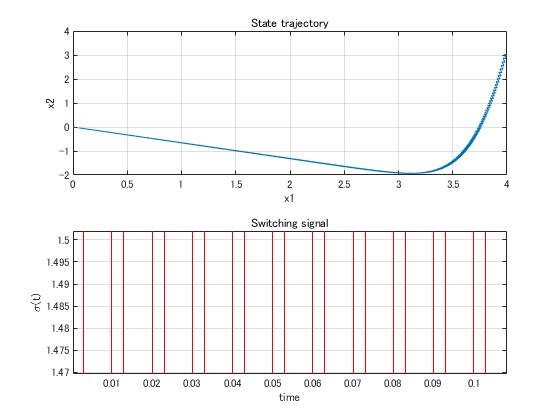
\includegraphics[width=0.7\linewidth]{./trajecctory_and_signal.jpg}
	\caption{システムの状態の軌跡とスイッチング信号}
	\label{fig-1}
\end{figure}

\end{document}
